\chapter{Project execution}
\textit{This chapter contains the explanation of the groups working and development methods.}
\section{Project approach}
The group seeks to work iteratively to constantly improve on the architecture and design. The project flow is illustrated on the figure \ref{fig:projectflow} below, which is also found in the preliminary project paper found on the enclosed CD \cite{cd}.
\begin{figure}[hbpt]
	\centering
	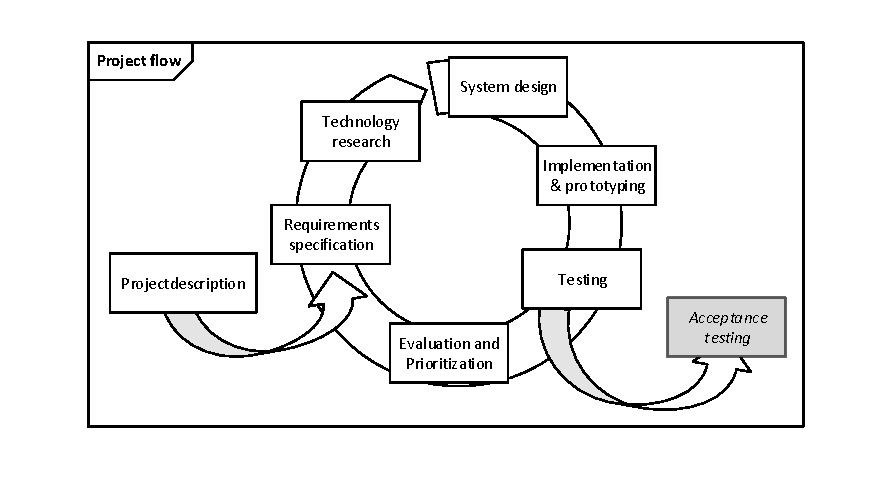
\includegraphics[width=1\textwidth]{billeder/9projectexecution/projectflow}
	\caption{Project flow}
	\label{fig:projectflow}
\end{figure}

This flow allows to redesign parts of the system which didn't work desirably. It also helps prioritize the parts that needs attention and downgrade phases of less importance or phases which has been fully formed.\\
An example of prioritization is the requirements specification phase which takes less and less time throughout the project because it simply isn't possible to keep making changes to it.\\
Another example is the prototyping part. Through multiple iterations there has been made a multitude of prototype print layouts. It is clear that the design and layout keeps improving.\\

\section{Work flow}
The work flow of the project follows a scrum-like behaviour. The central part of this  work flow is the project board. The board is used to structure work and progress. It is organized to give a good overview of the current tasks and upcoming tasks. A board meeting was held every work day with the following agenda:
\begin{itemize}
	\item What did I accomplish yesterday?
	\item What will I do today?
	\subitem $\circ$ Todays "Must-Win" battles?
	\item What obstacles are impeding my progress?
	\subitem $\circ$ What will help me overcome this?
\end{itemize}
The agenda insures forward momentum and consistent structure in the meetings.\\
The tasks are equipped with an estimated time consumption to prevent time spend on tasks getting out of hand. If a task stretches over one or more days, the time estimate is updated at each meeting to reflect progress and the future time consumption. An example of how the project board is structured is found in figure \ref{fig:prjboard}.

\begin{figure}[hbpt]
	\centering
	\includegraphics[width=0.8\textwidth]{billeder/9projectexecution/board}
	\caption{Project board}
	\label{fig:prjboard}
\end{figure}

Along with the daily meetings, supervisor meetings were held once every week. These meetings was build around the following agenda:
\begin{itemize}
	\item Since last meeting
	\item Present struggles/problems
	\item Next weeks goals
	\item Task related subjects
	\item Closing remarks
\end{itemize}

The supervisor meetings served to give both technical help as well as project guidance. These meetings enabled the supervisor to help the group move on if tasks seemed to be stuck or consuming too much time.

\section{Project planning}
The project is split into five phases. These phases serves as a linear progression from start to finish and plans which phases in the process to emphasize at what time in the project.\\
The phases used are only describing the actual work in a very rough manner. The phases are:
\begin{itemize}
	\item System design 
	\item Technology study 
	\item Development 
	\item Finalize documentation 
	\item Report 
	\label{it:phases}
\end{itemize}

The phases are used to make a rough time schedule throughout the project. In the time schedule each phase is given a specific duration. This duration reflects the extent of each phase and therefore how much time each phase required. The time schedule made in the preliminary project was modified a little during the project and the final time schedule is seen on figure \ref{fig:TimeSched}.

\begin{figure}[hbpt]
	\centering
	\includegraphics[width=0.7\textwidth]{billeder/9projectexecution/Timeschedule_neat}
	\caption{Time Schedule}
	\label{fig:TimeSched}
\end{figure}

These phases gave base for the documentation needed for the project. Below is seen a document tree describing the relationship between documents and project phases.

\begin{figure}[hbpt]
	\centering
	\includegraphics[width=.95\textwidth]{billeder/9projectexecution/documenttree}
	\caption{Document tree}
\end{figure}

Every artefact from this project has been subject to review atleast once. When a document was ready for review, it was through-read by each member of the group. A review meeting was held and a review document form was filled-out. The review document contained every information needed to correct the artefact under review. The review documents can be found on the enclosed CD \cite{cd}. The meeting facilitator had the responsibility to import the changes to the artefact.\\
Together with the review scheme, revision control of all documents, hardware and software is held to maintain traceability throughout the project. 
Hardware print layouts were also reviewed and all of the revisions were kept in order to evaluate the progress made on the hardware.

Throughout the project, every module and piece of hardware has been made in collaboration. This means there is no clear cut division of the project that has a specific stakeholder. The only division is the CDU software and the sensor node logic. This means that one person alone was responsible for the part but not that the other person could not have fulfilled the same task. On figure \ref{fig:workvenn} a venn diagram is shown to give a rough overview of the task/implementation distribution.

\begin{figure}[hbpt]
	\centering
	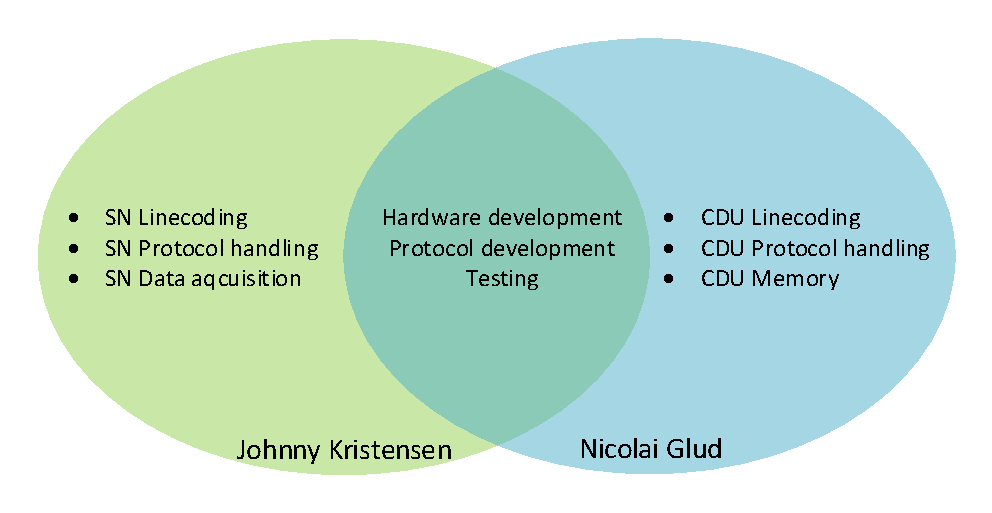
\includegraphics[width=.8\textwidth]{billeder/9projectexecution/workload_venn}
	\caption{Workload/distribution venn diagram}
	\label{fig:workvenn}
\end{figure}



%\section{Introduction}
%We started this project with a lot of knowledge from previous projects. This knowledge lead us to the methods of working that we used throughout the project. The whole project was separated into phases and put on a time schedule. The time schedule is found in figure \ref{fig:TimeSched}.
%\begin{figure}[H]
%\centering
%\includegraphics[width=0.8\textwidth]{billeder/Timeschedule_neat}
%\caption{Time Schedule}
%\label{fig:TimeSched}
%\end{figure}
%The phases we used are only describing the actual work in a very rough manner. These phases are:
%\begin{itemize}
%\item System design phase
%\item Technology study phase
%\item Development phase
%\item Finalize documentation phase
%\item Report phase
%\label{it:phases}
%\end{itemize}
%Each phase gave way to one of more documents. The tree of the phases and documents are found in figure \ref{fig:doctree}.
%\begin{figure}[H]
%\centering
%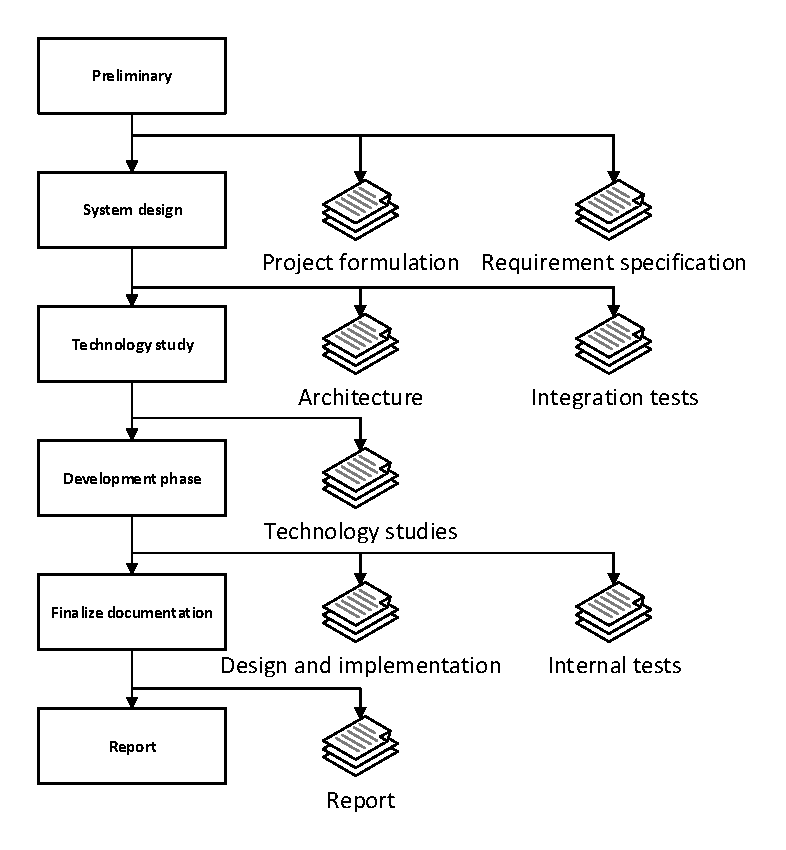
\includegraphics[width=0.6\textwidth]{billeder/DocumentTree}
%\caption{Document Tree and Phases}
%\label{fig:doctree}
%\end{figure}
%
%\section{Work method}
%A project board was used to keep track of current and future tasks. The board is heavily inspired by the scrum principle. Every day a board meeting was held with the following agenda:
%\begin{itemize}
%\item What did I accomplish yesterday?
%\item What will I do today?
%\subitem $\circ$ Todays "Must-Win" battles?
%\item What obstacles are impeding my progress?
%\subitem $\circ$ What will help me overcome this?
%\end{itemize}
%The tasks are equipped with an estimated time consumption. If a task stretches over 1 or more days, the time estimate is updated to reflect the future time consumption. An example of how the project board is structure is found in figure \ref{fig:prjboard}.
%\begin{figure}[H]
%\centering
%\includegraphics[width=0.8\textwidth]{billeder/board}
%\caption{Project board}
%\label{fig:prjboard}
%\end{figure}
%
%Every week a meeting with the project supervisor was held. The meeting was structured in the following way:
%\begin{itemize}
%\item Since last meeting
%\item Present struggles/problems
%\item Next weeks goals
%\item Workrelated subjects
%\item Closing remarks
%\end{itemize}
%
%Every artefact from this project has been review atleast once. When a document was ready for review, it was through-read by each member of the group. Notes was put in separate copies and a review meeting was held. Durre discusing the meeting the notes wesed and the things that needed to be changed was put into a review document. This way it is easy to see which changes were made in which revision of the document. 
%
%Hardware print layouts were also reviewed and all of the revisions were kept in order to evaluate the progress made on the hardware.
%
%Throughout the project, every module or piece of hardware has been made in collaboration. The means there is no clear cut division of the project that has a specific stakeholders. The only division is the CDU software and the sensor node logic. This means that one person alone was responsible for the part but not that the other person could not have fulfilled the same task.
%
